% ---------- Metadata ----------
\title[Aula 7]{Aula 7 - Título da Aula}
\author[Marcato]{Professor: André L. Marcato}
\institute[UFJF]{Universidade Federal de Juiz de Fora \\ Engenharia Elétrica — Robótica e Automação Industrial}

% ---------- Title ----------
\begin{frame}
  \titlepage
\end{frame}

% ---------- Overview ----------
\begin{frame}{Roteiro}
\tableofcontents
\end{frame}

% ---------- Conteúdo ----------
\section{Conceitos de Interfaces}

% --- Slide: Por que interfaces próprias? ---
\begin{frame}[fragile]{\href{https://docs.ros.org/en/humble/Tutorials/Beginner-Client-Libraries/Custom-ROS2-Interfaces.html}{\uline{Interfaces Próprias (.msg, .srv, .action)}}}
  \begin{itemize}
    \item O ROS 2 fornece tipos padrão (\texttt{std\_msgs}, \texttt{geometry\_msgs}, etc.), mas nem sempre são suficientes.
    \item \textbf{Custom Interfaces}: Permitem criar estruturas de dados específicas para seu robô.
    \item \textbf{Boa prática}: Criar um \textbf{pacote dedicado} apenas para interfaces (ex: \texttt{my\_robot\_interfaces}).
      \begin{itemize}
        \item Facilita dependências (vários nós podem usar as mesmas mensagens).
        \item Evita erros de compilação cíclica.
      \end{itemize}
  \end{itemize}
\end{frame}

% --- Slide: Fluxo de Geração (Diagrama) ---
\begin{frame}{Fluxo de Geração de Interfaces}
  \centering
  % Diagrama mostrando: Arquivo Texto (.msg) -> Compilador (rosidl) -> Código (Python/C++)
  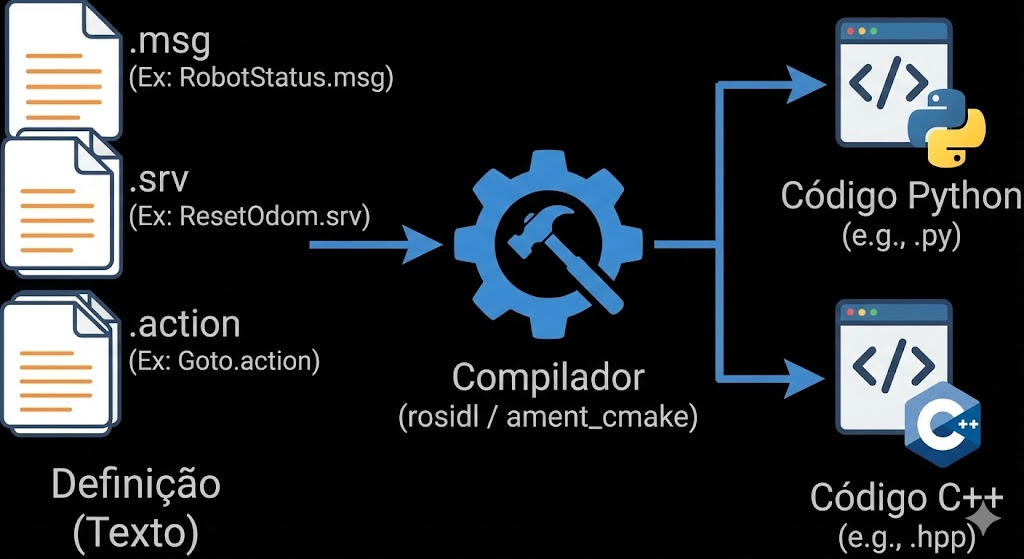
\includegraphics[width=0.9\textwidth]{aula7/images/interface_generation_flow.png}
\end{frame}

% --- Slide: Estrutura dos Arquivos ---
\begin{frame}[fragile]{Estrutura dos Arquivos}
  \textbf{Mensagem (.msg)}
  \begin{center}
  
\includegraphics[width=0.65\textwidth]{code_robot_status_msg.png}
  \end{center}

  \textbf{Serviço (.srv)}
  \begin{center}
  
\includegraphics[width=0.65\textwidth]{code_reset_odom_srv.png}
  \end{center}

  \textbf{Action (.action)}
  \begin{center}
  
\includegraphics[width=0.65\textwidth]{code_goto_action.png}
  \end{center}
\end{frame}


\section{Criando o Pacote de Interfaces}

% --- Slide: Configuração do Pacote (CMake) ---
\begin{frame}[fragile]{Configuração: Pacote CMake}
  \begin{itemize}
    \item Interfaces requerem um pacote \textbf{ament\_cmake} (mesmo se você usar Python nos nós).
  \end{itemize}
  
\begin{lstlisting}[style=bashstyle]
$ ros2 pkg create --build-type ament_cmake my_interfaces
$ mkdir msg srv action
\end{lstlisting}

  \vspace{0.5em}
  \textbf{package.xml (Adições necessárias)}:
  \begin{center}
  
\includegraphics[width=0.95\textwidth]{code_package_xml_interfaces.png}
  \end{center}
\end{frame}

% --- Slide: Configuração CMakeLists.txt ---
\begin{frame}[fragile]{Configuração: CMakeLists.txt}
  \begin{itemize}
    \item Devemos instruir o compilador a gerar os códigos Python/C++ a partir dos arquivos de texto.
  \end{itemize}

  \begin{center}
  
\includegraphics[width=0.95\textwidth]{code_cmake_interfaces.png}
  \end{center}
\end{frame}


\section{Uso no Código (Python)}

% --- Slide: Dependência no Nó (Client) ---
\begin{frame}[fragile]{Usando em outro pacote (Python)}
  \begin{itemize}
    \item Para usar suas mensagens no pacote do robô (\texttt{my\_robot\_py}), adicione a dependência no \texttt{package.xml} dele:
  \end{itemize}

  \begin{center}
  
\includegraphics[width=0.95\textwidth]{code_package_xml_depend.png}
  \end{center}

  \begin{itemize}
    \item No código Python, a importação segue a estrutura da pasta:
  \end{itemize}

  \begin{center}
  
\includegraphics[width=0.95\textwidth]{code_python_interfaces.png}
  \end{center}
\end{frame}


\section{Prática}

% --- Slide: Passo a Passo 1 ---
\begin{frame}[fragile]{Prática — Criar e Compilar (1/2)}
  \textbf{1. Criar pacote de interfaces}
\begin{lstlisting}[style=bashstyle]
$ cd ~/ros2_ws/src
$ ros2 pkg create --build-type ament_cmake my_interfaces
$ cd my_interfaces
$ mkdir msg srv
# Crie msg/HardwareStatus.msg:
#   int64 temperature
#   bool are_motors_ready
#   string debug_message
\end{lstlisting}

  \textbf{2. Ajustar XML e CMake}
  \begin{itemize}
    \item Adicione as tags no \texttt{package.xml} e a função \texttt{rosidl\_generate\_interfaces} no \texttt{CMakeLists.txt} (como visto nos slides anteriores).
  \end{itemize}
\end{frame}

% --- Slide: Passo a Passo 2 ---
\begin{frame}[fragile]{Prática — Criar e Compilar (2/2)}
  \textbf{3. Compilar Interfaces}
  \begin{itemize}
    \item É vital compilar o pacote de interfaces \textbf{antes} de tentar usá-lo.
  \end{itemize}
\begin{lstlisting}[style=bashstyle]
$ cd ~/ros2_ws
$ colcon build --packages-select my_interfaces
$ source install/setup.bash
\end{lstlisting}

  \textbf{4. Verificar Geração}
\begin{lstlisting}[style=bashstyle]
$ ros2 interface show my_interfaces/msg/HardwareStatus
# Deve imprimir:
# int64 temperature
# bool are_motors_ready
# string debug_message
\end{lstlisting}
\end{frame}

% --- Slide: Exercício Final ---
\begin{frame}[fragile]{Exercício Final}
  \begin{block}{Publisher Customizado}
    Crie um nó Python simples (em outro pacote) que publica uma mensagem \texttt{HardwareStatus} a cada 1 segundo.
  \end{block}
  \begin{enumerate}
    \item Crie/Use um pacote Python (\texttt{my\_robot\_py}).
    \item Adicione \texttt{<depend>my\_interfaces</depend>} no \texttt{package.xml}.
    \item No código:
      \begin{itemize}
        \item \texttt{from my\_interfaces.msg import HardwareStatus}
        \item Preencha \texttt{msg.temperature} com um valor aleatório.
        \item Publique no tópico \texttt{/hardware\_status}.
      \end{itemize}
    \item Verifique com \texttt{ros2 topic echo /hardware\_status}.
  \end{enumerate}
\end{frame}

